\documentclass[11pt]{article}

\usepackage[margin=1in]{geometry}
\usepackage{parskip}
\usepackage{amssymb}
\usepackage{xcolor}
\usepackage{listings}
\usepackage{booktabs}
\usepackage{tikz}
\usetikzlibrary{shapes.geometric, shapes.symbols, arrows.meta, positioning, fit, backgrounds, calc, decorations.pathreplacing}
\usepackage[hidelinks,
            pdftitle={Pylon 8891 RCA: V3 Extract Async Union Misresolution},
            pdfauthor={Sravan Puttagunta},
            pdfsubject={Reducto Python SDK -- AsyncJobResponseResult union picks PipelineResponse for v3 payloads}]{hyperref}

% --- color palette ----------------------------------------------------------
\definecolor{good}{HTML}{2A8C4A}
\definecolor{goodbg}{HTML}{D4F1DC}
\definecolor{bad}{HTML}{C0392B}
\definecolor{badbg}{HTML}{FADBD8}
\definecolor{neutral}{HTML}{2C3E50}
\definecolor{neutralbg}{HTML}{EAEDED}
\definecolor{accent}{HTML}{1F6FB2}
\definecolor{accentbg}{HTML}{D6EAF8}
\definecolor{warn}{HTML}{B7950B}
\definecolor{warnbg}{HTML}{FCF3CF}

% --- code listings ----------------------------------------------------------
\definecolor{codebg}{HTML}{F5F5F5}
\definecolor{codekey}{HTML}{0033B3}
\definecolor{codestr}{HTML}{067D17}
\definecolor{codecmt}{HTML}{8C8C8C}

\lstdefinestyle{py}{
    basicstyle=\ttfamily\small,
    backgroundcolor=\color{codebg},
    keywordstyle=\color{codekey}\bfseries,
    stringstyle=\color{codestr},
    commentstyle=\color{codecmt}\itshape,
    showstringspaces=false,
    breaklines=true,
    frame=single,
    rulecolor=\color{codebg},
    framesep=4pt,
    xleftmargin=4pt,
    xrightmargin=4pt,
    language=Python,
    morekeywords={Optional,Union,List,Literal,TypeAlias,BaseModel},
    columns=fullflexible,
    keepspaces=true,
}

\lstdefinestyle{shell}{
    basicstyle=\ttfamily\small,
    backgroundcolor=\color{codebg},
    showstringspaces=false,
    breaklines=true,
    frame=single,
    rulecolor=\color{codebg},
    framesep=4pt,
    xleftmargin=4pt,
    xrightmargin=4pt,
    columns=fullflexible,
    keepspaces=true,
}

% --- TikZ shared styles -----------------------------------------------------
\tikzset{
    box/.style={rectangle, rounded corners=4pt, draw=neutral, line width=1pt,
                minimum width=3cm, minimum height=1.4cm, align=center, font=\small,
                inner sep=4pt},
    goodbox/.style={box, fill=goodbg, draw=good},
    badbox/.style={box, fill=badbg, draw=bad},
    accentbox/.style={box, fill=accentbg, draw=accent},
    warnbox/.style={box, fill=warnbg, draw=warn},
    neutralbox/.style={box, fill=neutralbg, draw=neutral},
    decision/.style={diamond, draw=neutral, fill=warnbg, line width=1pt, aspect=2,
                     align=center, font=\small, inner sep=2pt},
    note/.style={font=\footnotesize\itshape, text=neutral},
    arr/.style={-Stealth, line width=0.9pt, color=neutral},
    badarr/.style={-Stealth, line width=1.4pt, color=bad},
    goodarr/.style={-Stealth, line width=1.4pt, color=good, dashed},
}

% ===========================================================================
\begin{document}

\begin{flushleft}
{\LARGE\bfseries Root Cause Analysis: Pylon \#8891}\\[2pt]
{\large V3 Extract Async Response Misresolution in \texttt{reducto-python-sdk}}
\end{flushleft}

\vspace{4pt}
\begin{tabular}{@{}ll@{}}
\textbf{Customer}        & Kalepa (reporter: Ewa Juralewicz) \\
\textbf{Pylon issue}     & \#8891 -- ``Intermittent parsing failures after update'' \\
\textbf{First reported}  & 2026-04-13 \\
\textbf{RCA prepared}    & 2026-05-05 by Sravan Puttagunta \\
\textbf{Affected SDK}    & \texttt{reductoai} v0.13.0 (customer); reproduces on v0.22.0 (current \texttt{main}) \\
\textbf{Trigger}         & API repo PR \#5420 (2026-04-24) \\
\textbf{Severity}        & Medium -- silent data loss on the typed path \\
\end{tabular}

% ---------------------------------------------------------------------------
\section{Executive Summary}

After API PR \#5420 began returning v3-shaped \texttt{result} objects unconditionally, customers polling \texttt{/job/\{job\_id\}} via the Stainless-generated Python SDK started seeing empty extracted results. The SDK deserializes the inner \texttt{AsyncJobResponseResult} union to the wrong variant: \textbf{\texttt{PipelineResponse}}, not \texttt{V3Extract}. Customers' typed access path reads \texttt{None} while the actual extracted data is preserved as untyped extras on a \texttt{Result} instance.

The thread's prior hypothesis -- first sketched by Alvin and later restated by Thomas (who flagged it as not yet validated) -- located the bug in Stainless's order-dependent loose \texttt{construct()} fallback, blaming the position of \texttt{ExtractResponse} ahead of \texttt{V3Extract}. Reproduction shows that path is never reached. Pydantic's smart-union validation succeeds at the very top of \texttt{construct\_type} and selects \texttt{PipelineResponse} because the SDK's regenerated \texttt{Result} model has all-optional fields combined with the SDK's default \texttt{extra="allow"}.

The upstream cause is a Stainless code-generation footgun: the server-side \texttt{PipelineResult} declares \texttt{parse}, \texttt{extract}, and \texttt{split} as \texttt{T | None} with no default (\emph{required-but-nullable}), but Stainless regenerates them as \texttt{Optional[T] = None} (\emph{optional-with-default}), dropping the constraint that the keys must be present. The bug therefore lives entirely in the regenerated SDK; the server's own \texttt{model\_validate} dispatch loop in \texttt{handlers/job.py} is correct because it uses the un-translated server types.

The bug is specific to the async polling path. The sync endpoint's response is cast through a different, two-member union (\texttt{Union[V3Extract, AsyncExtractResponse]}) that does not include \texttt{PipelineResponse}, so smart-union resolves to \texttt{V3Extract} cleanly -- which is why the customer reported the failure was much more frequent on the async endpoint and worked around it by switching to sync.

\textbf{One-place fix.} Add a \texttt{Literal} discriminator field to each variant in \texttt{AsyncJobResponseResult} (server-side, in \texttt{src/config/internal.py}). The OpenAPI export carries the discriminator through to Stainless, which generates a Pydantic discriminated union. The SDK's \texttt{construct\_type} discriminator-dispatch path runs before smart-union scoring; field counts and \texttt{extra="allow"} stop affecting routing. The same change also lets the server's order-dependent \texttt{model\_validate} loop be replaced with a direct \texttt{AsyncJobResponse.model\_validate(...)} call. The discriminator-on-\texttt{V3Extract}-only branch \texttt{alvin/fix-v3-extract-sdk-discriminator} does not work because Pydantic discriminator dispatch requires every variant to expose the same field.

% ---------------------------------------------------------------------------
\section{Variant Resolution Outcome (Visual)}

\begin{center}
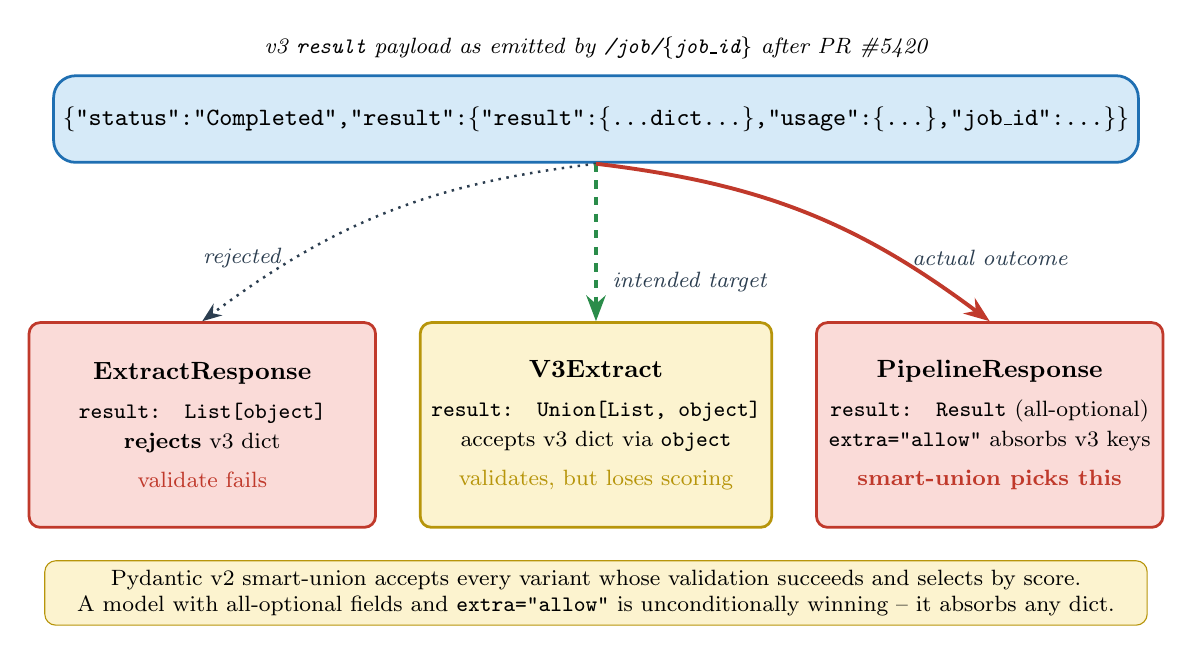
\begin{tikzpicture}[node distance=0.6cm and 0.8cm]

  \node[draw, fill=accentbg, rounded corners=8pt, minimum width=10cm, minimum height=1.1cm,
        align=center, font=\small\ttfamily, draw=accent, line width=1pt] (pkg)
        {\{"status":"Completed","result":\{"result":\{...dict...\},"usage":\{...\},"job\_id":...\}\}};
  \node[font=\footnotesize\itshape, above=2pt of pkg.north, anchor=south]
        {v3 \texttt{result} payload as emitted by \texttt{/job/\{job\_id\}} after PR \#5420};

  % Three variants
  \node[badbox, below=2.0cm of pkg, xshift=-5cm, minimum width=4.4cm, minimum height=2.6cm] (er)
        {\textbf{ExtractResponse}\\[3pt]
         \footnotesize \texttt{result: List[object]}\\
         \footnotesize \textbf{rejects} v3 dict\\[3pt]
         \footnotesize\textcolor{bad}{validate fails}};

  \node[warnbox, below=2.0cm of pkg, minimum width=4.4cm, minimum height=2.6cm] (v3)
        {\textbf{V3Extract}\\[3pt]
         \footnotesize \texttt{result: Union[List, object]}\\
         \footnotesize accepts v3 dict via \texttt{object}\\[3pt]
         \footnotesize\textcolor{warn}{validates, but loses scoring}};

  \node[badbox, below=2.0cm of pkg, xshift=5cm, minimum width=4.4cm, minimum height=2.6cm] (pr)
        {\textbf{PipelineResponse}\\[3pt]
         \footnotesize \texttt{result: Result} (all-optional)\\
         \footnotesize \texttt{extra="allow"} absorbs v3 keys\\[3pt]
         \footnotesize\textcolor{bad}{\textbf{smart-union picks this}}};

  \draw[arr, color=neutral, dotted] (pkg.south) to[bend right=15] node[note, near end, left=2pt]{rejected} (er.north);
  \draw[goodarr] (pkg.south) -- node[note, near end, right=2pt]{intended target} (v3.north);
  \draw[badarr]  (pkg.south) to[bend left=15] node[note, near end, right=2pt]{actual outcome} (pr.north);

  \node[draw, fill=warnbg, draw=warn, rounded corners=4pt, below=0.4cm of v3,
        minimum width=14cm, align=center, font=\footnotesize] (verdict)
        {Pydantic v2 smart-union accepts every variant whose validation succeeds and selects by score.\\
         A model with all-optional fields and \texttt{extra="allow"} is unconditionally winning -- it absorbs any dict.};

\end{tikzpicture}
\end{center}

The relevant code: \texttt{src/reducto/types/shared/pipeline\_response.py:43--58}.

\begin{lstlisting}[style=py]
class Result(BaseModel):
    extract: Optional[ResultExtract] = None
    parse:   Optional[ResultParse]   = None
    split:   Optional[SplitResponse] = None
    edit:    Optional[EditResponse]  = None

class PipelineResponse(BaseModel):
    job_id: str
    result: Result
    usage:  ParseUsage
\end{lstlisting}

The inner \texttt{Result} validates against any dict because every field is optional with a default and the SDK's \texttt{BaseModel} sets \texttt{extra="allow"} (\texttt{src/reducto/\_models.py:110}). The customer's \texttt{company\_name} / \texttt{total\_amount} keys land on the \texttt{Result} as untyped extras; the four typed accessors stay \texttt{None}.

% ---------------------------------------------------------------------------
\section{Decision Flow in \texttt{construct\_type} (Visual)}

\begin{center}
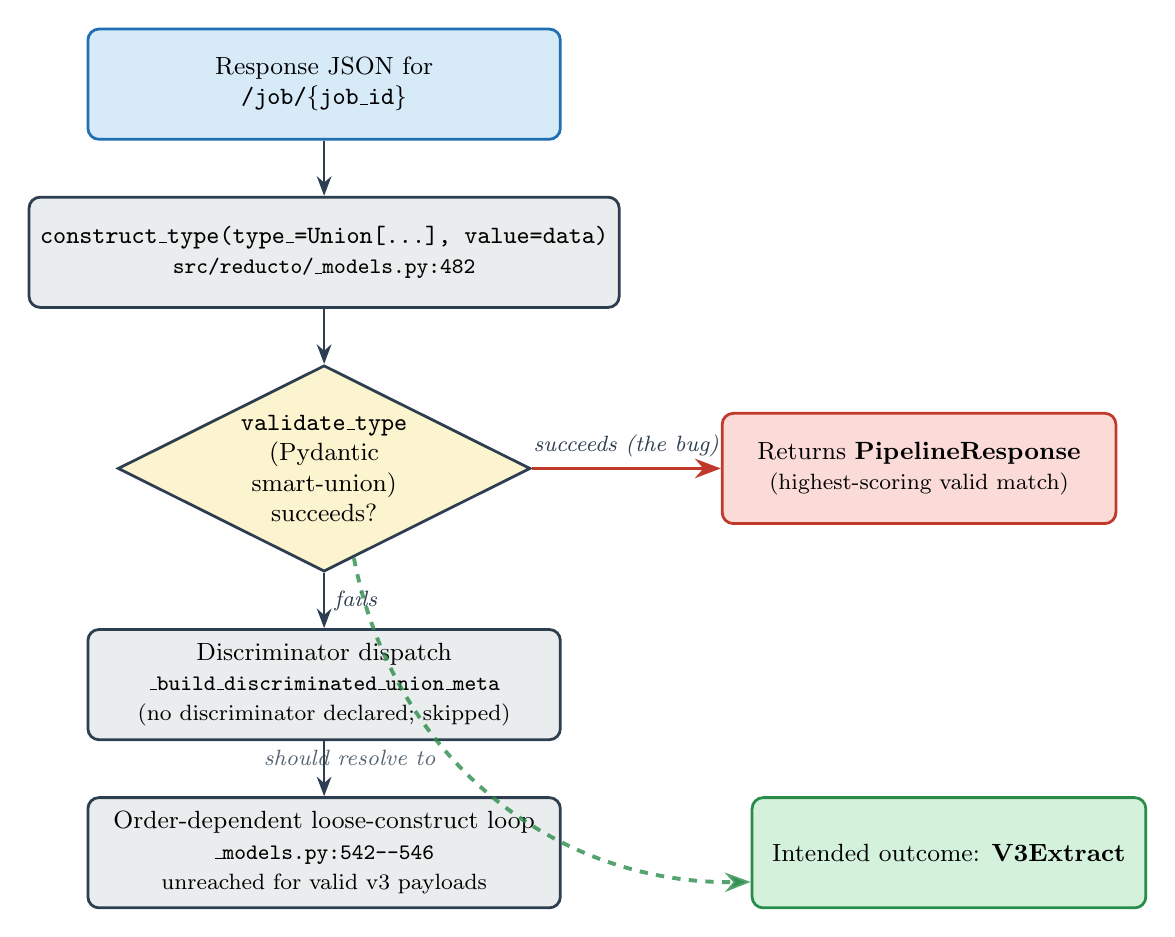
\begin{tikzpicture}[node distance=0.7cm]

  \node[accentbox, minimum width=6cm] (start)
        {Response JSON for\\\texttt{/job/\{job\_id\}}};

  \node[neutralbox, below=of start, minimum width=6cm] (call)
        {\texttt{construct\_type(type\_=Union[\dots], value=data)}\\\footnotesize\texttt{src/reducto/\_models.py:482}};

  \node[decision, below=of call, minimum width=4.6cm, minimum height=1.4cm] (val)
        {\texttt{validate\_type}\\(Pydantic\\smart-union)\\succeeds?};

  \node[badbox, right=2.4cm of val, minimum width=5.0cm] (won)
        {Returns \textbf{PipelineResponse}\\\footnotesize(highest-scoring valid match)};

  \node[neutralbox, below=of val, minimum width=6cm] (disc)
        {Discriminator dispatch\\\footnotesize\texttt{\_build\_discriminated\_union\_meta}\\\footnotesize(no discriminator declared; skipped)};

  \node[neutralbox, below=of disc, minimum width=6cm] (loop)
        {Order-dependent loose-construct loop\\\footnotesize\texttt{\_models.py:542--546}\\\footnotesize unreached for valid v3 payloads};

  \node[goodbox, right=2.4cm of loop, minimum width=5.0cm] (good)
        {Intended outcome: \textbf{V3Extract}};

  \draw[arr] (start) -- (call);
  \draw[arr] (call) -- (val);
  \draw[badarr] (val) -- node[note, above]{succeeds (the bug)} (won);
  \draw[arr] (val) -- node[note, right]{fails} (disc);
  \draw[arr] (disc) -- (loop);
  \draw[goodarr, opacity=0.8] (val) to[bend right=40] node[note, left=2pt, pos=0.4]{should resolve to} (good);

\end{tikzpicture}
\end{center}

The thread's prior hypothesis reasoned about the loose-construct loop at the bottom of the diagram. That loop runs only when every variant raises during strict validation. For valid v3 payloads, smart-union resolution succeeds at the top and short-circuits the rest of the function. Reordering the union or adding a discriminator only to \texttt{V3Extract} cannot change which path the bug is on.

% ---------------------------------------------------------------------------
\section{Regression Anchor: Before vs After PR \#5420 (Visual)}

\begin{center}
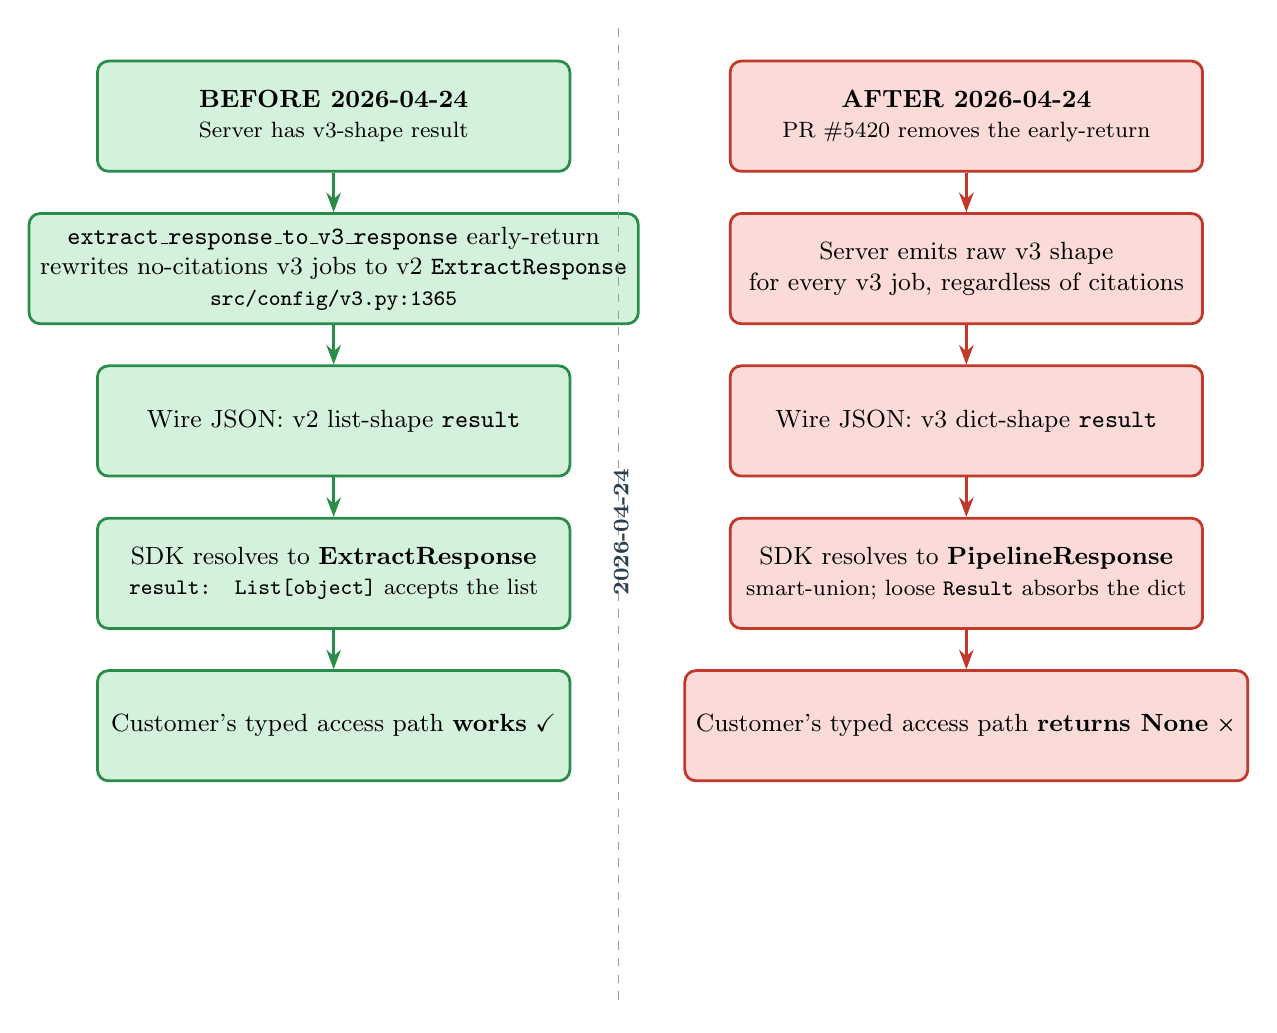
\begin{tikzpicture}[node distance=0.5cm]

  \node[goodbox, minimum width=6cm] (b1) {\textbf{BEFORE 2026-04-24}\\\footnotesize Server has v3-shape result};
  \node[goodbox, below=of b1, minimum width=6cm] (b2)
       {\texttt{extract\_response\_to\_v3\_response} early-return\\rewrites no-citations v3 jobs to v2 \texttt{ExtractResponse}\\\footnotesize\texttt{src/config/v3.py:1365}};
  \node[goodbox, below=of b2, minimum width=6cm] (b3)
       {Wire JSON: v2 list-shape \texttt{result}};
  \node[goodbox, below=of b3, minimum width=6cm] (b4)
       {SDK resolves to \textbf{ExtractResponse}\\\footnotesize\texttt{result: List[object]} accepts the list};
  \node[goodbox, below=of b4, minimum width=6cm] (b5)
       {Customer's typed access path \textbf{works} \checkmark};

  \node[badbox, right=2cm of b1, minimum width=6cm] (a1) {\textbf{AFTER 2026-04-24}\\\footnotesize PR \#5420 removes the early-return};
  \node[badbox, below=of a1, minimum width=6cm] (a2)
       {Server emits raw v3 shape\\for every v3 job, regardless of citations};
  \node[badbox, below=of a2, minimum width=6cm] (a3)
       {Wire JSON: v3 dict-shape \texttt{result}};
  \node[badbox, below=of a3, minimum width=6cm] (a4)
       {SDK resolves to \textbf{PipelineResponse}\\\footnotesize smart-union; loose \texttt{Result} absorbs the dict};
  \node[badbox, below=of a4, minimum width=6cm] (a5)
       {Customer's typed access path \textbf{returns None} \texttimes};

  \draw[arr, color=good] (b1) -- (b2);
  \draw[arr, color=good] (b2) -- (b3);
  \draw[arr, color=good] (b3) -- (b4);
  \draw[arr, color=good] (b4) -- (b5);

  \draw[arr, color=bad] (a1) -- (a2);
  \draw[arr, color=bad] (a2) -- (a3);
  \draw[arr, color=bad] (a3) -- (a4);
  \draw[arr, color=bad] (a4) -- (a5);

  \draw[dashed, color=neutral!50] ($(b1.north east)+(0.6,0.4)$) -- ($(b1.north east)+(0.6,-12)$);
  \node[font=\footnotesize\bfseries, color=neutral, rotate=90, anchor=south] at ($(b1.north east)+(0.85,-6)$) {2026-04-24};

\end{tikzpicture}
\end{center}

% ---------------------------------------------------------------------------
\section{Customer-Visible Symptom}

\begin{quote}\itshape
``Started suddenly reading your results as empty from async endpoint (but not all). In the studio it seems like schema is correct but in our code which has not changed and uses 0.13.0 version of your sdk in Python started suddenly wrongly parsing the responses.''
\end{quote}
\hfill --- Ewa Juralewicz, 2026-04-13 10:57

Studio renders correctly because it consumes the raw JSON server-side. The customer's Python code consumes the SDK-deserialized object, and the typed accessor path returns \texttt{None}. The data is present on the underlying object as untyped extras; nothing in the SDK surfaces the discrepancy.

% ---------------------------------------------------------------------------
\section{Reproduction}

A regression test at \texttt{tests/test\_pylon\_8891\_v3\_async\_union.py} (committed on branch \texttt{sravan/repro-pylon-8891}) exercises the same path as \texttt{client.job.get(job\_id)}. The file contains four classes of tests:
\begin{itemize}
  \item Four async-path bug tests marked \texttt{@pytest.mark.xfail(strict=True)} -- they fail on \texttt{main} today; once the fix lands they begin passing and the strict mode forces removal of the marker, turning them into permanent regression checks.
  \item One sync positive control verifying \texttt{ExtractRunResponse} resolves correctly today and guarding against future spec changes that introduce a permissive variant on the sync side.
  \item Two snapshot tests pinning the SDK-side \texttt{Result} permissiveness -- they pass today (documenting the lossy-translation outcome) and start failing once the spec is tightened, signaling that the snapshots can be deleted.
  \item One proof-of-concept demonstrating the recommended discriminator fix routes correctly even when the variants remain individually permissive.
\end{itemize}

Core async-path assertion:

\begin{lstlisting}[style=py]
from reducto._models import construct_type
from reducto.types.job_get_response import AsyncJobResponse, AsyncJobResponseResult

v3_inner = {
    "result": {
        "company_name": {"value": "Acme Corp", "citations": [...]},
        "total_amount": {"value": 1234.56, "citations": [...]},
    },
    "usage": {"num_fields": 2, "num_pages": 2},
    "job_id": "ee9734ef-...",
    "studio_link": "...",
}
payload = {"status": "Completed", "progress": 1.0, "result": v3_inner}
obj = construct_type(type_=AsyncJobResponse, value=payload)
\end{lstlisting}

Output on \texttt{main} at v0.22.0:

\begin{lstlisting}[style=shell]
inner AsyncJobResponseResult union resolution:
  validate_python succeeded -> PipelineResponse
  loose construct loop (each variant in declared union order):
    ParseResponse      -> ParseResponse
    ExtractResponse    -> ExtractResponse
    SplitResponse      -> SplitResponse
    EditResponse       -> EditResponse
    PipelineResponse   -> PipelineResponse
    V3Extract          -> V3Extract
    ClassifyResponse   -> ClassifyResponse

AsyncJobResponse + v3 payload:
  outer  : AsyncJobResponse
  result : PipelineResponse
  inner Result typed values: extract=None, parse=None, split=None, edit=None
  inner Result extra keys (customer data, not typed): ['company_name', 'total_amount']
\end{lstlisting}

Two relevant facts:
\begin{enumerate}
  \item Strict \texttt{validate\_python} on the union succeeds; the loose-construct fallback is never entered.
  \item In the unreached fallback, every variant constructs without raising. The first declared variant wins by definition; that variant is \texttt{ParseResponse}, not \texttt{ExtractResponse}.
\end{enumerate}

% ---------------------------------------------------------------------------
\section{Where the Routing Logic Lives}

The decision ``what kind of response is this?'' happens at three sites, only one of which is the actual bug:

\textbf{Site 1 -- Server wire-time conversion} (\texttt{api/src/config/v3.py:1332}). \texttt{extract\_response\_to\_v3\_response} decides whether an extract result goes out as v2 \texttt{ExtractResponse} or v3 \texttt{V3ExtractResponse}. After PR \#5420 (2026-04-24), this passes through as v2 only in the narrow ``no citations \emph{and} no confidence \emph{and} \texttt{generate\_citations=False}'' case. For Kalepa (citations enabled), the v3 shape is emitted. \emph{Behaving as designed.}

\textbf{Site 2 -- Server S3 reload} (\texttt{api/src/handlers/job.py:90--147}). When \texttt{/job/\{job\_id\}} retrieves a completed job's JSON from S3, it walks an ordered list of response types and calls \texttt{model\_validate} on each:

\begin{lstlisting}[style=py]
for response_type in [
    ParseResponse, ExtractResponse, SplitResponse, EditResponse,
    PipelineResponse, V3ExtractResponse, ClassifyResponse,
]:
    try:
        result = response_type.model_validate(json_result)
        return AsyncJobResponse(status="Completed", result=result)
    except pydantic.ValidationError:
        continue
\end{lstlisting}

This loop superficially resembles the SDK's order-dependent fallback, but it is \emph{not} broken. The server-side \texttt{PipelineResult} (\texttt{src/config/internal.py:1132--1138}) declares \texttt{parse}, \texttt{extract}, and \texttt{split} as \texttt{T | None} \emph{without defaults} -- required-but-nullable -- so a v3 extract job's JSON, which has none of those keys, fails \texttt{PipelineResponse.model\_validate} and the loop correctly proceeds to \texttt{V3ExtractResponse}. \emph{Behaving correctly.}

\textbf{Site 3 -- SDK response deserialization} (\texttt{src/reducto/\_models.py:482--548}). \texttt{construct\_type} runs Pydantic smart-union over the regenerated \texttt{AsyncJobResponseResult}. The SDK's \texttt{Result} model has \texttt{= None} on every field, so a v3 dict validates against it; smart-union scoring then selects \texttt{PipelineResponse} over \texttt{V3Extract}. \textbf{This is the bug.}

A spec-level discriminator on \texttt{AsyncJobResponseResult} variants in \texttt{api/src/config/internal.py} fixes Site~3 by propagating through OpenAPI to Stainless, and it simplifies Site~2 (the loop reduces to one \texttt{AsyncJobResponse.model\_validate} call). One change, both sites converge on structural dispatch instead of scoring.

% ---------------------------------------------------------------------------
\section{Root Cause}

\subsection{Deserialization path}

\texttt{client.job.get(...)} returns through \texttt{\_BaseClient.\_process\_response\_data} (\texttt{src/reducto/\_base\_client.py:649--671}). With the default \texttt{\_strict\_response\_validation=False}, line 669 invokes:

\begin{lstlisting}[style=py]
return cast(ResponseT, construct_type(type_=cast_to, value=data))
\end{lstlisting}

For union-typed fields, \texttt{construct\_type} (\texttt{src/reducto/\_models.py:482--548}) attempts strict union validation first, then a discriminator dispatch, then an order-dependent loose-construct loop:

\begin{lstlisting}[style=py]
if is_union(origin):
    try:
        return validate_type(type_=..., value=value)   # smart-union
    except Exception:
        pass
    # discriminator dispatch (no discriminator on this union; skipped)
    for variant in args:
        try:
            return construct_type(value=value, type_=variant)
        except Exception:
            continue
\end{lstlisting}

\texttt{validate\_type} dispatches into \texttt{pydantic.TypeAdapter(union).validate\_python(value)}. Pydantic v2's default smart-union mode runs every variant through validation, scores the matches, and returns the highest-scoring one. The fallback loop runs only when every variant raises.

\subsection{Why \texttt{PipelineResponse} wins}

\texttt{PipelineResponse.result} is a \texttt{Result} model with four \texttt{Optional} fields, each defaulting to \texttt{None}. The SDK's \texttt{BaseModel} configures \texttt{extra="allow"}, so any dict validates against \texttt{Result}: unknown keys are absorbed onto the instance, known keys default. The remaining \texttt{PipelineResponse} fields (\texttt{job\_id: str}, \texttt{usage: ParseUsage}) match shapes that overlap with the v3 payload.

\texttt{ExtractResponse.result} is typed \texttt{List[object]} -- a v3 dict fails strict validation, so this variant is excluded.

\texttt{V3Extract.result} is typed \texttt{Union[List[object], object]} and validates the dict via the \texttt{object} arm. It is a structurally valid match for the payload but loses the smart-union scoring race to \texttt{PipelineResponse}, which presents as a more ``complete'' nested model.

\subsection{The Stainless lossy translation}

The all-\texttt{Optional}-with-defaults shape of the SDK's \texttt{Result} is not what the server-side spec declares. In \texttt{api/src/config/internal.py:1132}:

\begin{lstlisting}[style=py]
class PipelineResult(BaseModel):
    parse:   ParseResponse | list[ParseResponse] | None                       # no default
    extract: list[ExtractSplitResponse] | ExtractResponse | V3ExtractResponse | None  # no default
    split:   SplitResponse | None                                             # no default
    edit:    EditResponse | None = None                                       # default present
\end{lstlisting}

Three of the four fields have \emph{no default}. In Pydantic v2 this means ``required-but-nullable'': an inbound JSON object must contain those keys, but \texttt{null} is a valid value. \texttt{PipelineResult.model\_validate(\{\})} fails on the server because \texttt{parse}, \texttt{extract}, and \texttt{split} are missing.

Stainless regenerates the same model into the SDK as:

\begin{lstlisting}[style=py]
class Result(BaseModel):
    extract: Optional[ResultExtract] = None
    parse:   Optional[ResultParse]   = None
    split:   Optional[SplitResponse] = None
    edit:    Optional[EditResponse]  = None
\end{lstlisting}

Every field gains \texttt{= None}. The SDK contract becomes ``optional-with-default,'' which is strictly weaker: \texttt{Result.model\_validate(\{\})} now succeeds. Combined with the SDK's \texttt{extra="allow"} default, the regenerated \texttt{Result} validates against \emph{any} dict, which is precisely what hands a v3 payload to the smart-union scorer as a candidate \texttt{PipelineResponse}.

This is a generic Stainless / OpenAPI-export footgun: a server type expressing ``required-nullable'' via \texttt{T | None} without a default does not survive code generation as the same constraint. The defensive options are (a) avoid the pattern in spec-exported types, (b) introduce a discriminator field that survives regeneration as a load-bearing structural element, or (c) regression-test the regenerated SDK for unintended optionality. Two snapshot tests in \texttt{tests/test\_pylon\_8891\_v3\_async\_union.py} pin the current SDK shape so any future spec tightening trips them as a signal.

\subsection{Why the sync endpoint is unaffected}

The customer reported that ``frequency is much higher on async endpoint compared to sync one'' (Ewa, 2026-04-13 10:38). The asymmetry is entirely about which variants populate each union.

\textbf{Sync path.} \texttt{client.extract.run(...)} casts to \texttt{ExtractRunResponse} (\texttt{src/reducto/types/extract\_run\_response.py:11}):

\begin{lstlisting}[style=py]
ExtractRunResponse: TypeAlias = Union[V3Extract, AsyncExtractResponse]
\end{lstlisting}

This union has two members and \emph{no \texttt{PipelineResponse}}. \texttt{AsyncExtractResponse} is just \texttt{\{job\_id: str\}} -- it's the immediate ack returned when an async submission is accepted. Smart-union scoring picks \texttt{V3Extract} for v3 payloads cleanly because \texttt{V3Extract} matches the full shape (\texttt{result}, \texttt{usage}, \texttt{job\_id}, \texttt{studio\_link}) while \texttt{AsyncExtractResponse} matches only \texttt{job\_id}. The customer's data lands on the typed path.

\textbf{Async path.} \texttt{client.job.get(job\_id)} casts to \texttt{JobGetResponse}, whose inner \texttt{AsyncJobResponseResult} union contains seven variants \emph{including} \texttt{PipelineResponse}:

\begin{lstlisting}[style=py]
AsyncJobResponseResult = Union[
    ParseResponse, ExtractResponse, SplitResponse, EditResponse,
    PipelineResponse, V3Extract, ClassifyResponse, None,
]
\end{lstlisting}

Once \texttt{PipelineResponse} is in the union, smart-union has the option to pick its loose \texttt{Result} model -- and does. The bug is therefore unique to the async polling path. Same payload shape on the wire; different cast type; different winner.

\subsection{Why this regressed when it did}

Before API PR \#5420 (2026-04-24), \texttt{extract\_response\_to\_v3\_response} (\texttt{src/config/v3.py:1365}) early-returned the v2 \texttt{ExtractResponse} shape when no citations were present. The wire JSON was a v2-style list, which validated cleanly against \texttt{ExtractResponse}. PR \#5420 removed that early-return; v3 jobs now serialize as their native dict shape unconditionally, exposing the smart-union ambiguity above.

% ---------------------------------------------------------------------------
\section{Why the Prior Hypothesis Was Incomplete}

The thread's prior diagnosis -- first sketched by Alvin, later restated by Thomas (who flagged it as not yet validated) -- pointed at the order \texttt{[ExtractResponse, ..., V3Extract]} in \texttt{AsyncJobResponseResult}. The claim was that Stainless's loose \texttt{construct()} would pick \texttt{ExtractResponse} first and fill its required \texttt{citations} with a default \texttt{[]}.

Three points where that account doesn't survive reproduction:
\begin{enumerate}
  \item Strict validation succeeds and short-circuits the loose-construct loop. The order-dependent code path is unreached for valid v3 payloads.
  \item In the loop, every variant in the union constructs without raising, so the \emph{first} listed variant is the winner. That is \texttt{ParseResponse}, not \texttt{ExtractResponse}; reordering the latter two has no effect on the fallback result.
  \item \texttt{ExtractResponse.citations} is declared \texttt{Optional[List[object]] = None} (\texttt{src/reducto/types/shared/extract\_response.py:12}), not a required field with default \texttt{[]}. A spurious top-level field would deserialize to \texttt{null}, not \texttt{[]}.
\end{enumerate}

The branch \texttt{alvin/fix-v3-extract-sdk-discriminator} adds \texttt{response\_type: Literal["v3"] = "v3"} to \texttt{V3Extract} only. \texttt{construct\_type} consults discriminator metadata via \texttt{\_build\_discriminated\_union\_meta} (\texttt{\_models.py:651}), which requires every variant in the union to expose the same discriminator field. Adding it to one variant does not enable the discriminator path, and even if it did, smart-union still selects \texttt{PipelineResponse} for any payload missing the discriminator.

% ---------------------------------------------------------------------------
\section{Remediation}

\subsection{Recommended: spec-level discriminator (one place, both sites)}

In \texttt{api/src/config/internal.py}, add a \texttt{Literal} discriminator field to each variant of \texttt{AsyncJobResponseResult} and wrap the union with \texttt{pydantic.Discriminator}:

\begin{lstlisting}[style=py]
class V3ExtractResponse(BaseModel):
    response_type: Literal["v3_extract"] = "v3_extract"
    # ... existing fields

class PipelineResponse(BaseModel):
    response_type: Literal["pipeline"] = "pipeline"
    # ... existing fields

# similarly for ParseResponse, ExtractResponse, SplitResponse, EditResponse, ClassifyResponse

class AsyncJobResponse(BaseModel):
    status: Literal["Pending", "Completed", "Failed", "Idle"]
    result: Annotated[
        ParseResponse | ExtractResponse | SplitResponse | EditResponse |
        PipelineResponse | V3ExtractResponse | ClassifyResponse,
        Discriminator("response_type"),
    ] | None = None
\end{lstlisting}

Effects:
\begin{itemize}
  \item \textbf{Server runtime.} \texttt{handlers/job.py:116--147} can be replaced by a single \texttt{AsyncJobResponse.model\_validate(...)} call -- Pydantic dispatches via the discriminator. The current ordered loop becomes structurally honest dispatch and stops being a hidden source of routing decisions.
  \item \textbf{OpenAPI export.} Pydantic emits a JSON Schema \texttt{discriminator: \{ propertyName: response\_type, mapping: \{...\} \}} block. Stainless preserves this.
  \item \textbf{SDK regeneration.} Stainless generates a Pydantic discriminated union. \texttt{construct\_type}'s discriminator-dispatch path (\texttt{src/reducto/\_models.py:533--539}) runs before smart-union scoring. The all-\texttt{Optional} \texttt{Result} model becomes irrelevant to routing because routing is now structural, not score-based. Field counts and \texttt{extra="allow"} cease to matter.
  \item \textbf{Wire format.} Every response carries \texttt{"response\_type": "..."}. Additive change; clients that ignore unknown fields are unaffected.
  \item \textbf{Legacy S3 JSON.} Existing job results lack the \texttt{response\_type} key, but the \texttt{Literal} field has a default value, so \texttt{model\_validate} backfills it. No migration needed.
\end{itemize}

The proof-of-concept test \texttt{test\_proposed\_discriminator\_fix\_routes\_v3\_correctly} in the repro PR demonstrates that a discriminated union with deliberately permissive variants still dispatches correctly.

\subsection{Alternates (and why they are inferior)}

\begin{description}
  \item[Tighten \texttt{PipelineResult} via \texttt{model\_validator}.] Add a Pydantic model-level validator requiring at least one of \texttt{parse}/\texttt{extract}/\texttt{split} non-\texttt{None}. Pydantic-runtime only; does not propagate through OpenAPI to Stainless. The SDK would still smart-union into \texttt{Result} for any dict. To make it propagate would require hand-written \texttt{json\_schema\_extra} emitting an \texttt{anyOf} constraint -- brittle and unlikely to survive regen cleanly.

  \item[Drop \texttt{PipelineResponse} from \texttt{AsyncJobResponseResult}.] Smallest spec change; correctness contingent on a routing audit that confirms pipelines never legitimately surface here. Even if true, the union structure remains a smart-union magnet for any future variant introduced under similar conditions.

  \item[SDK-side \texttt{model\_validator} workaround on a non-generated mixin.] Pre-resolves to \texttt{V3Extract} based on shape inspection. Survives Stainless regen but ships only if we need a release before the spec change can round-trip. Once the discriminator is in place, this becomes dead code.

  \item[Reorder the union or add a discriminator only to \texttt{V3Extract} (\texttt{alvin/fix-v3-extract-sdk-discriminator}).] Does not address the actual mechanism. Smart-union scoring -- not declaration order -- is what selects \texttt{PipelineResponse}, and Pydantic discriminator dispatch requires every variant to expose the same field.
\end{description}

\subsection{Action sequence}

\begin{enumerate}
  \item Land the spec change in \texttt{api/src/config/internal.py}: discriminators on each variant, \texttt{Annotated[..., Discriminator(...)]} on the union.
  \item Replace \texttt{handlers/job.py:116--147}'s ordered loop with a single \texttt{AsyncJobResponse.model\_validate(json\_result)} call. Verify against historical job IDs, including Kalepa's \texttt{ee9734ef-...}.
  \item Regenerate the SDK via Stainless. Confirm the regenerated union carries the discriminator.
  \item In the SDK PR (this repo), remove the four \texttt{xfail} markers from \texttt{tests/test\_pylon\_8891\_v3\_async\_union.py}. The two snapshot tests pinning \texttt{Result}'s permissiveness should also start failing; delete them or invert as the spec change supersedes their purpose.
  \item Cut the SDK release. Notify Kalepa they can move back to async polling.
\end{enumerate}

% ---------------------------------------------------------------------------
\section{Detection \& Prevention}

\begin{itemize}
  \item \textbf{Detection gap.} Smart-union resolution to \texttt{PipelineResponse} happens silently. No log line, no warning, no validation error. The customer's only signal is downstream typed-accessor reads of \texttt{None}. A debug-mode warning in \texttt{construct\_type} when union resolution accepts a value with $\geq N$ surplus extras would have surfaced this immediately.
  \item \textbf{Watch for Stainless lossy translation.} Server-side \texttt{T | None} without a default is the OpenAPI/JSON-Schema idiom for ``required-but-nullable.'' Stainless drops the constraint on regen, emitting \texttt{Optional[T] = None}. Audit any spec-exported model that uses this pattern; consider replacing with discriminated unions or required-field constraints expressed in JSON Schema directly. Running \texttt{T.model\_validate(\{\})} on each generated model is a fast snapshot check.
  \item \textbf{Spec hygiene.} Any union member whose regenerated Pydantic model has all-optional fields combined with \texttt{extra="allow"} is a smart-union magnet. Treat that combination as a lint failure on the regenerated SDK, since spec-level ``required-nullable'' alone is not load-bearing through code generation.
  \item \textbf{Process: reproduce before broadcasting.} The thread's prior diagnosis circulated for three weeks without being run against a payload. Phase 1 of systematic debugging -- reproduce on a representative input before posting an RCA -- catches this.
\end{itemize}

% ---------------------------------------------------------------------------
\section{Timeline}

\begin{description}
  \item[2026-04-13 10:21] Kalepa reports intermittent empty parsing results on the async endpoint. Studio renders the failing job IDs correctly, indicating a client-side deserialization issue rather than server compute.
  \item[2026-04-13 17:58] Sid Pagariya posts API PR \#5238 (later abandoned) and notes possible v3 vs.\ v2 response-typing breakage.
  \item[2026-04-13 20:27] Alvin Ryanputra summarizes a hypothesis: union ordering of \texttt{ExtractResponse} before \texttt{V3ExtractResponse} causes \texttt{construct()} to pick \texttt{ExtractResponse} and fill \texttt{citations} with a default \texttt{[]}.
  \item[2026-04-15 08:30] Customer is told to ignore top-level \texttt{citations} for now; they switch to the sync endpoint and resume normal traffic.
  \item[2026-04-24] API PR \#5420 (\texttt{94fce175b}) merges, removing the early-return in \texttt{extract\_response\_to\_v3\_response} (\texttt{src/config/v3.py:1365}). Every v3 job now serializes as native v3 shape on the wire.
  \item[2026-05-05] Thomas Boser posts a written-up version of the same union-order theory plus a proposed fix path: (1) land discriminator, (2) reorder unions, (3) regen Stainless. He explicitly notes ``\emph{i haven't validated this at all}.''
  \item[2026-05-05] Sravan reproduces the bug on \texttt{main}; the actual variant picked is \texttt{PipelineResponse}, not \texttt{ExtractResponse}.
\end{description}

% ---------------------------------------------------------------------------
\section{Artifacts}

\begin{itemize}
  \item Regression test: \texttt{tests/test\_pylon\_8891\_v3\_async\_union.py} in \texttt{reducto-python-sdk}, branch \texttt{sravan/repro-pylon-8891}.
  \item Worktree: \texttt{.claude/worktrees/fix-v3-extract-top-level-citations} (off \texttt{main} at v0.22.0).
  \item Related (unmerged, does not fix): API repo branch \texttt{alvin/fix-v3-extract-sdk-discriminator}, commit \texttt{362d9dc99}.
  \item Triggering commit: API repo \texttt{94fce175b} (PR \#5420, 2026-04-24).
  \item Pylon thread: \#cus-kalepa, issue \#8891.
\end{itemize}

\end{document}
